\documentclass{lecture}
\input{command}
\graphicspath{{./Discrete-Time/}}

\course{Stochastic Thermodynamics and Machine Learning}{2023/4}{Prof.~Max Welling}
\note{Chapter 2}{Graphical Models and Latent Variables}{\today}

\usepackage{tikz}
\usetikzlibrary{shapes,arrows,positioning,calc}

\begin{document}
\makeheader

\section{Latent Variable Models}
The whole book will center around the idea that we have models with observed variables $\bx$ and unobserved (latent) variables $\bz$. These unobserved variables in physics equal the detailed positions and momenta of the particles. (In subsequent chapters, when we are describing physical systems with position and momenta we use the notation: $\bze=(\bx,\bp)$.)

In physics, there are typically three levels of variables:
\begin{enumerate}
	\item[1.] Observations, which are typically macroscopic quantities we can measure with our sensors, e.g., temperature and pressure.
	\item[2.] The unobserved (latent) positions and momenta of the atoms, which undergo random evolution.
	\item[3.] The degrees of freedom of a heat bath with many particles that interact with (e.g., collide with) the molecules of the system we study. They are causing the Brownian motion-like behavior of the molecules.
\end{enumerate}
In AI, we also have observed variables (our data) and unobserved variables (the many degrees of the world we do not track). While we usually do not consider a heat bath of particles interacting with our latent variables and causing them to be stochastic, we do formulate probability distributions over latent variables to quantify what we do (and do not) know about them.

A latent variable model (LVM) is defined as follows:
\begin{align}
	p_X(\bx) = \sum_{\bz} p_{X|Z}(\bx|\bz)~p_Z(\bz). \label{eqn:lvm}
\end{align}
We will assume discrete states, but if we include continuous states, we can simply replace sums with integrals. The subscripts indicate that the function $p_X$ does not have to be the same as $p_Z$. However, these subscripts are cumbersome, and if we can see that they are different from their arguments, we will omit them in the following. Note that the marginal distribution $p_X$ is given as a marginalization over $\bz$ (a mixture over $\bz$), which makes this model class very expressive!

Using Bayes' rule, we can now define a number of other interesting distributions,
\begin{align}
	 &\text{Likelihood:}~ p(\bx|\bz),\\
	 &\text{Joint:}~p(\bx,\bz)=p(\bx|\bz)p(\bz),\\
	 &\text{Marginal:}~p(\bx) = \sum_{\bz} p(\bx|\bz)~p(\bz),\\
	 &\text{Prior:}~p(\bz) = \sum_\bx p(\bx,\bz) = \left[\sum_{\bx} p(\bx|\bz)\right]~p(\bz),\\
	 &\text{Posterior:}~p(\bz|\bx) = \frac{p(\bx,\bz)}{p(\bx)}=\frac{p(\bx|\bz)p(\bz)}{p(\bx)}. \label{eqn:posterior}
\end{align}

As an example, consider a model where the prior $p_Z$ is given by a Gaussian density, and the conditionals are also Gaussian,
\begin{align}
	p(\bz) = G(\bzero,\eI),~~~p(\bx|\bz)=G(\bW\bz,\bSig). \label{eqn:gaussian_example}
\end{align}
You can now compute the joint distribution
\begin{align}
	 &p(\bx,\bz) = G(\bzero,\bGa),\\
	 &\bGa^{-1}=\left[\begin{array}{cc}
			                  \bSig^{-1}       & -\bSig^{-1}\bW           \\
			                  -\bW^T\bSig^{-1} & \eI + \bW^T\bSig^{-1}\bW
		                  \end{array}\right]. \label{eqn:joint_gaussian}
\end{align}
And from here, we can derive the posterior distribution by ``completing squares'',
\begin{align}
	 &p(\bz|\bx) = G(\bmu,\bLa),\\
	 &\bLa^{-1} = \eI + \bW^T\bSig^{-1}\bW, \label{eqn:posterior_precision}\\
	 &\bmu = \bLa \bW^T\bSig^{-1}\bx. \label{eqn:posterior_mean}
\end{align}
As an exercise, you can try to derive \cref{eqn:posterior_precision,eqn:posterior_mean} from \cref{eqn:gaussian_example,eqn:joint_gaussian}.

We can interpret this model as Factor Analysis, where the factors of variation are given by $\bz$, and the posterior will tell us which factors explain most of the signal in the observations $\bx$.


\section{Graphical Models}

\begin{figure}[ht]
	\centering
	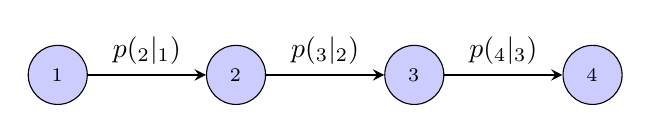
\begin{tikzpicture}[
			node distance=1.5cm,
			observed/.style={circle, draw, fill=blue!20, minimum size=0.75cm},
			latent/.style={circle, draw, fill=red!20, minimum size=0.75cm},
			arrow/.style={->, >=stealth, thick}
		]
		% Define nodes
		\node[observed] (1) {$\bx_1$};
		\node[observed] (2) [right=of 1] {$\bx_2$};
		\node[observed] (3) [right=of 2] {$\bx_3$};
		\node[observed] (4) [right=of 3] {$\bx_4$};

		% Draw arrows
		\draw[arrow] (1) -- node[above] {$p(\bx_2|\bx_1)$} (2);
		\draw[arrow] (2) -- node[above] {$p(\bx_3|\bx_2)$} (3);
		\draw[arrow] (3) -- node[above] {$p(\bx_4|\bx_3)$} (4);
	\end{tikzpicture}
	\caption{Graphical Model of a Markov Chain representing the probability distribution $p(\bx_1,\ldots,\bx_4) = p(\bx_1)\prod_{t=2}^4 p(\bx_t|\bx_{t-1})$. The arrows indicate the sequential dependency between variables in a simple linear progression. Blue nodes represent observed variables. This structure encodes the Markov property, where each variable depends only on the immediately preceding variable.}
	\label{fig:markov_chain}
\end{figure}


We can now start to put structure on these models. The field that deals with structured (latent variable) models is called Graphical Models (GM)~\cite{Koller2009Probabilistic}. In a GM, nodes represent random variables, and edges represent the probabilistic dependencies between these variables. The structure of the graph encodes the conditional independence assumptions made by the model.

To give an example that we will encounter frequently in this book, let us consider Markov Models (MM) given by the structured distribution:
\begin{align}
	p(\bx_0,\ldots,\bx_T) = p_0(\bx_0)\prod_{t=1}^T p_t(\bx_t|\bx_{t-1}),
\end{align}
where each conditional distribution $p_t(\bx_t|\bx_{t-1})$ can be different for every time step. Each GM makes certain assumptions about the (conditional) independence between random variables. In the MM above, the assumption is that $\bx_t\perp \bx_0,\ldots,\bx_{t-2}~|~\bx_{t-1},~~\forall t$. In words: the variable $\bx_t$ is statistically independent of all variables in the past of $\bx_t$ given the value of $\bx_{t-1}$. A simple proof can be given as follows:
\begin{align}
	p(\bx_t,\bx_{t-2}|\bx_{t-1}) = \frac{p(\bx_t|\bx_{t-1})p(\bx_{t-1}|\bx_{t-2})p(\bx_{t-2})}{p(\bx_{t-1})} = p(\bx_t|\bx_{t-1}) p(\bx_{t-2}|\bx_{t-1}),
\end{align}
where we have marginalized out all the variables $\bx_0,\ldots,\bx_{t-3},\bx_{t+1},\ldots,\bx_T$ and we used Bayes' rule to get to the last equation. The result states precisely the conditional independence relation as claimed: the conditional distribution over $\bx_t$ and $\bx_{t-2}$ factorizes if we are given $\bx_{t-1}$.


\paragraph{Hidden Markov Model}
An example of a Markov Model with latent variables is given by the Hidden Markov Model (HMM)~\cite{Rabiner1989Tutorial}:
\begin{align}
	p(\bx_0,\ldots,\bx_T,\bz_0,\ldots,\bz_T)=p_0(\bz_0)\prod_{t=1}^T p_t(\bz_t|\bz_{t-1})~\prod_{t=0}^T p(\bx_t|\bz_t),
\end{align}
where $\bz_t$ are the latent variables and $\bx_t$ are the observed variables at time step $t$. You can draw a node for every variable and an arrow for every conditional distribution, which visualizes the structure of the model and from which you can actually read off all the conditional independence relations, as shown in \cref{fig:hmm}.

\begin{figure}[ht]
	\centering
	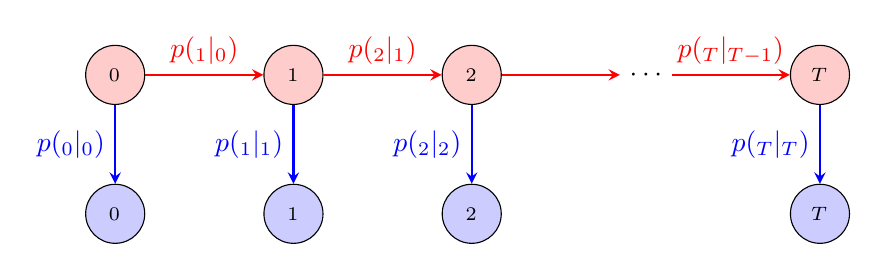
\begin{tikzpicture}[
			node distance=1.5cm,
			observed/.style={circle, draw, fill=blue!20, minimum size=0.75cm},
			latent/.style={circle, draw, fill=red!20, minimum size=0.75cm},
			arrow/.style={->, >=stealth, thick}
		]
		% Define nodes
		\node[latent] (Z0) {$\bz_0$};
		\node[latent] (Z1) [right=of Z0] {$\bz_1$};
		\node[latent] (Z2) [right=of Z1] {$\bz_2$};
		\node (dots) [right=of Z2] {$\cdots$};
		\node[latent] (ZT) [right=of dots] {$\bz_T$};

		\node[observed] (X0) [below=1.0cm of Z0] {$\bx_0$};
		\node[observed] (X1) [below=1.0cm of Z1] {$\bx_1$};
		\node[observed] (X2) [below=1.0cm of Z2] {$\bx_2$};
		\node[observed] (XT) [below=1.0cm of ZT] {$\bx_T$};

		% Draw arrows
		\draw[arrow, red] (Z0) -- node[above] {$p(\bz_1|\bz_0)$} (Z1);
		\draw[arrow, red] (Z1) -- node[above] {$p(\bz_2|\bz_1)$} (Z2);
		\draw[arrow, red] (Z2) -- (dots);
		\draw[arrow, red] (dots) -- node[above] {$p(\bz_T|\bz_{T-1})$} (ZT);

		\draw[arrow, blue] (Z0) -- node[left] {$p(\bx_0|\bz_0)$} (X0);
		\draw[arrow, blue] (Z1) -- node[left] {$p(\bx_1|\bz_1)$} (X1);
		\draw[arrow, blue] (Z2) -- node[left] {$p(\bx_2|\bz_2)$} (X2);
		\draw[arrow, blue] (ZT) -- node[left] {$p(\bx_T|\bz_T)$} (XT);
	\end{tikzpicture}
	\caption{Graphical model representation of a Hidden Markov Model (HMM). The model structure is defined by the probability distribution $p(\bx_0,\ldots,\bx_T,\bz_0,\ldots,\bz_T)=p_0(\bz_0)\prod_{t=1}^T p_t(\bz_t|\bz_{t-1})~\prod_{t=0}^T p(\bx_t|\bz_t)$. Red arrows represent transition probabilities between latent states, while blue arrows represent emission probabilities from latent states to observed variables. Red nodes denote latent variables, and blue nodes denote observed variables. This structure captures the temporal dependencies in the latent process and the conditional independence of observations given the latent states.}
	\label{fig:hmm}
\end{figure}



\paragraph{Markov Random Fields}
A final example that will be very useful for us are Markov Random Fields (MRF)~\cite{Kindermann1980Markov}. An MRF is defined in terms of potential functions over subsets of variables (both observed and unobserved). These potentials are typically defined locally in some space, i.e., they define who are neighbors of each other in this space. If we introduce cluster $\cG_\al$ as the cluster indexed by $\al$, and $\bx_\al=\{\bx_{\al(1)},\ldots,\bx_{\al(n_\al)}\}$ as the subset of variables that participate in that cluster, we can define the following probability distribution:
\begin{align}
	p(\bx_1,\ldots,\bx_N)= \frac{1}{Z}\exp\left(\sum_\al \Phi_\al(\bx_\al)\right).
\end{align}
where $\Phi_\al(\bx_\al)$ are the potential functions defined over the clusters, and $Z$ is the partition function.
We call this an undirected GM as we do not have conditional probability distributions but rather a type of Boltzmann distribution with structured potentials. We note that the exact same definition is used when we use a mix of latent variables $\bz$ and observed variables $\bx$. An example of an MRF is shown in \cref{fig:mrf}.

The conditional probability relations implied by the models are given by the following. First draw an (undirected) edge between a variable $\bx_i$ and all the variables that are in the same argument of some potential. Call this set the Markov Blanket (MB) $\cM(i)$ of variable $i$. We now have the conditional independence: $\bx_i\perp \bx_{\backslash i\cup\cM(i)}~|~\bx_{\cM(i)}$. In words: $\bx_i$ is independent of all other variables in the MRF outside the MB if we condition on the variables in the MB, or, the MB shields $\bx_i$ from statistical dependencies of the rest of the variables.

\begin{figure}[ht]
	\centering
	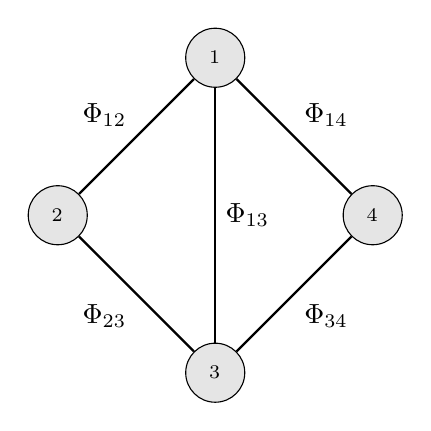
\begin{tikzpicture}[
			node distance=1.5cm,
			var/.style={circle, draw, fill=gray!20, minimum size=0.75cm},
			edge/.style={-, thick}
		]
		% Define nodes
		\node[var] (x1) at (0, 2) {$\bx_1$};
		\node[var] (x2) at (-2, 0) {$\bx_2$};
		\node[var] (x3) at (0, -2) {$\bx_3$};
		\node[var] (x4) at (2, 0) {$\bx_4$};

		% Draw edges
		\draw[edge] (x1) -- node[above left] {$\Phi_{12}$} (x2);
		\draw[edge] (x1) -- node[right] {$\Phi_{13}$} (x3);
		\draw[edge] (x1) -- node[above right] {$\Phi_{14}$} (x4);
		\draw[edge] (x2) -- node[below left] {$\Phi_{23}$} (x3);
		\draw[edge] (x3) -- node[below right] {$\Phi_{34}$} (x4);
	\end{tikzpicture}
	\caption{Markov Random Field (MRF) model representing the probability distribution $p(\bx_1,\ldots,\bx_4)= \frac{1}{Z}\exp\left(\sum_{(i,j)\in\mathcal{C}} \Phi_{ij}(\bx_i,\bx_j)\right)$, where $\mathcal{C}$ is the set of all cliques in the graph. The edges represent the pairwise potential functions $\Phi_{ij}$ defined over the neighboring variables $\bx_i$ and $\bx_j$, which form the cliques in the graph. In this example, the cliques are the pairs of connected nodes: $\{(1,2), (1,3), (1,4), (2,3), (3,4)\}$. Green nodes represent variables that can be either observed or latent. This structure encodes local dependencies and global constraints through the potential functions defined over the cliques.}
	\label{fig:mrf}
\end{figure}

\section{Variational EM Algorithm}

\begin{figure}[ht]
	\centering
	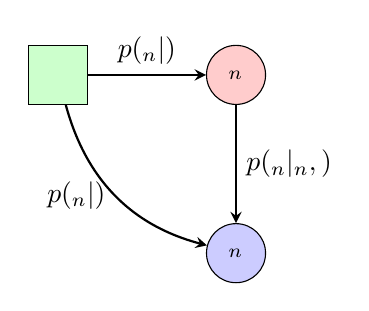
\begin{tikzpicture}[
			node distance=1.5cm,
			observed/.style={circle, draw, fill=blue!20, minimum size=0.75cm},
			latent/.style={circle, draw, fill=red!20, minimum size=0.75cm},
			param/.style={rectangle, draw, fill=green!20, minimum size=0.75cm},
			arrow/.style={->, >=stealth, thick}
		]
		% Define nodes
		\node[latent] (zn) {$\bz_n$};
		\node[observed] (xn) [below=of zn] {$\bx_n$};
		\node[param] (theta) [left=of zn] {$\bta$};

		% Draw arrows
		\draw[arrow] (zn) -- node[right] {$p(\bx_n|\bz_n,\bta)$} (xn);
		\draw[arrow] (theta) -- node[above] {$p(\bz_n|\bta)$} (zn);
		\draw[arrow] (theta) to[bend right] node[left] {$p(\bx_n|\bta)$} (xn);
	\end{tikzpicture}
	\caption{Latent Variable Model with parameter $\bta$ representing the probability distribution $p(\bx_n,\bz_n|\bta)=p(\bx_n|\bz_n,\bta)p(\bz_n|\bta)$. The arrow from $\bta$ to $\bx_n$ indicates that the observed variable $\bx_n$ depends on the parameter $\bta$, while the arrow from $\bz_n$ to $\bx_n$ represents the conditional probability $p(\bx_n|\bz_n,\bta)$. Blue nodes represent observed variables, red nodes represent latent variables, and green nodes represent parameters. This structure illustrates the hierarchical nature of the model and the flow of dependencies from parameters to latent variables to observations.}
	\label{fig:lvm_with_param}
\end{figure}

Once we have defined a GM, we need to learn it from data. A dataset consists of $N$ data-points, where each data-point assigns values to all of the observed variables in the GM. The marginal log-likelihood that we want to maximize is given by,
\begin{align}
	L(X,\bta) &=\sum_{n=1}^N \log p(\bx_n)\\
	          &=\sum_{n=1}^N \sum_{\bz_n} q_n(\bz_n) \log \frac{p(\bx_n) q_n(\bz_n)}{q_n(\bz_n)}\\
	          &=\sum_{n=1}^N \sum_{\bz_n} q_n(\bz_n) \log \left( \frac{p(\bx_n|\bz_n)p(\bz_n) q_n(\bz_n)}{p(\bz_n|\bx_n) q_n(\bz_n)} \right)\\
	          &=\sum_{n=1}^N \sum_{\bz_n} q_n(\bz_n) (\log p(\bx_n,\bz_n) - \log q_n(\bz_n)) + \sum_n \KL[q_n(\bz_n)||p(\bz_n|\bx_n)]\\
	          &\geq -\sum_{n=1}^N \cF[q_n,p] \equiv -\cF[q_1,\ldots,q_N,p] \label{eqn:ELBO}
\end{align}
where $q_n(\bz_n)$ are variational distributions introduced for each data point $n$. The transition from the second to the third line is true because $p(\bx_n)=p(\bx_n|\bz_n)p(\bz_n)/p(\bz_n|\bx_n)$ is true for every value of $\bz_n$. We conclude that the log-likelihood, which is the natural objective to maximize, is lower bounded by $-\cF$ which can be interpreted as the total free energy of the system of $N$ data-points.

\subsection{VE-step}
To maximize $L$, we now iterate two steps: first, we minimize $\cF$ over the distributions $\{q_n\}$. One can choose to do partial minimizations, e.g., only minimize over a subset of the $\{q_n\}$ or minimize for only a few steps. We call this the VE-step of the inference algorithm and note for future references that this is like relaxing a physical system that is out of equilibrium towards equilibrium. Assume we have parameterized the inference distributions with data-case specific parameters, $\bvphi_n$: $q_n(\bz_n|\bvphi_n)$. We can then take the derivative of $\cF$ w.r.t. $\bvphi_n$ to get,
\begin{align}
	 &\bna_{\bvphi_n}\cF =\\
	 &\sum_{\bz_n} [\bna_{\bvphi_n}q_n(\bz_n|\bvphi_n)](\log p(\bx_n,\bz_n) - \log q_n(\bz_n|\bvphi_n)) - \sum_{\bz_n} q_n(\bz_n|\bvphi_n) \bna_{\bvphi_n}\log q_n(\bz_n|\bvphi_n)\\
	 &= \sum_{\bz_n} [q_n(\bz_n|\bvphi_n)\bna_{\bvphi_n}\log q_n(\bz_n|\bvphi_n)][\log p(\bx_n,\bz_n) - \log q_n(\bz_n|\bvphi_n)]\\
	 &\approx \frac{1}{S}\sum_{s:\bz_{sn}\sim q_n}\bna_{\bvphi_{sn}}\log q_n(\bz_{sn}|\bvphi_n)[\log p(\bx_n,\bz_{sn}) - \log q_n(\bz_{sn}|\bvphi_n)]
\end{align}
where in the last line we replace the sum with Monte Carlo samples drawn from $q_n$, and we used the following tricks:
\begin{align}
	 &\bna_{\bvphi_n}q_n(\bz_n|\bvphi_n) = q_n(\bz_n|\bvphi_n)\bna_{\bvphi_n}\log q_n(\bz_n|\bvphi_n)\\
	 &\sum_{\bz_n} q_n(\bz_n)\bna_{\bvphi_n}\log q_n(\bz_n) = \sum_{\bz_n} \bna_{\bvphi_n} q_n(\bz_n) = \bna_{\bvphi_n} \sum_{\bz_n}  q_n(\bz_n) = \bna_{\bvphi_n} 1 = 0
\end{align}
This is called a reinforce estimator~\cite{Williams1992Simple}. Unfortunately, it has very high variance if you use a Monte Carlo estimate by sampling from $q$ to compute the gradient.

\paragraph{Reparameterization Trick}
For some distributions, there is a very nice trick to reduce the variance of this estimator called the reparameterization trick~\cite{Kingma2014Autoencoding}. This works as follows (see \cref{fig:reparameterization_trick} for an illustration of how this trick transforms the computation graph to enable efficient gradient calculation). Consider we like to compute the derivative of an integral of the following form:
\begin{align}
	\na_\ta \int\dd z~ q(z|\ta) f(z),
\end{align}
and imagine we can perform a change of variables $z=g(\eps,\ta)$ such that
\begin{align}
	\int\dd z~ q(z|\ta)=\int\dd\eps~ p(\eps)
\end{align}
with $p$ an easy to sample from standard distribution. As an example, you can consider a Gaussian distribution, where we have
\begin{align}
	 &\int\dd z ~G(z|\mu,\sg) f(z)= \int\dd \eps~G(\eps|0,1) f(\mu+\sg\eps),\\
	 &z = g(\eps,\mu,\sg) = \mu + \sg\eps.
\end{align}
In one dimension, this can always be achieved but in higher dimensions, it may be hard to identify the transformation. We can now rewrite:
\begin{align}
	 &\na_\ta \int\dd z~ q(\bz|\ta) f(z) = \int\dd \eps~G(\eps|0,1)\na_\ta f(g(\eps,\ta))\approx \frac{1}{N}\sum_{n:\eps_n\sim G} \frac{\der f}{\der g}\na_\ta g(\eps_n,\ta).
\end{align}
This estimator has much better variance properties!

\begin{figure}[ht]
	\centering
	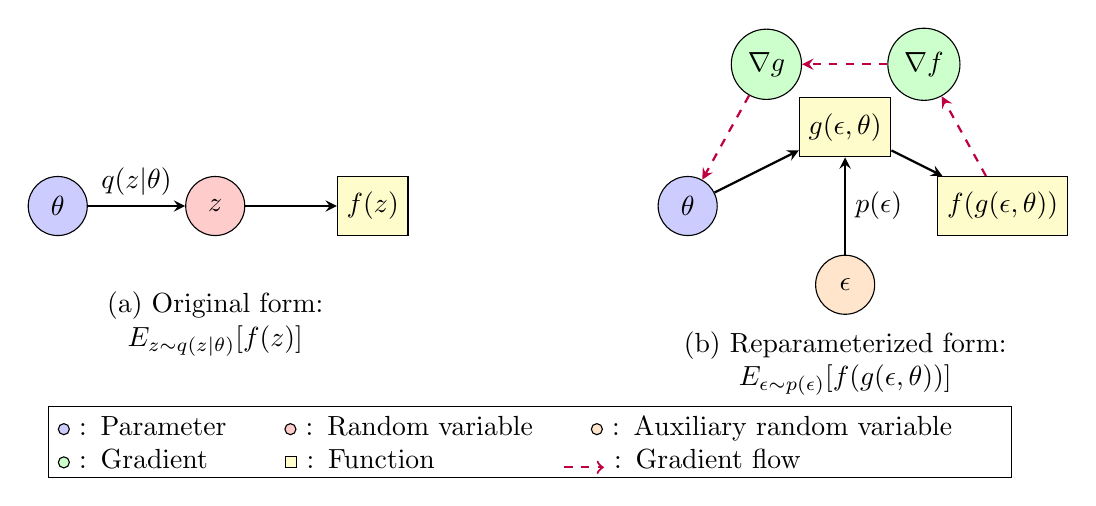
\begin{tikzpicture}[
			node distance=2cm,
			block/.style={rectangle, draw, fill=yellow!20, minimum size=0.75cm},
			circ/.style={circle, draw, minimum size=0.75cm},
			arrow/.style={->, >=stealth, thick},
			dashed arrow/.style={->, >=stealth, thick, dashed}
		]
		% Subfigure (a): Original form
		\begin{scope}[xshift=-4cm]
			\node[circ, fill=blue!20] (theta_a) at (0,0) {$\theta$};
			\node[circ, fill=red!20] (z_a) at (2,0) {$z$};
			\node[block] (f_a) at (4,0) {$f(z)$};
			\draw[arrow] (theta_a) -- node[above] {$q(z|\theta)$} (z_a);
			\draw[arrow] (z_a) -- (f_a);
			\node[text width=4cm, align=center] at (2,-1.5) {(a) Original form:\\
				$\mathbb{E}_{z \sim q(z|\theta)}[f(z)]$};
		\end{scope}
		% Subfigure (b): Reparameterized form
		\begin{scope}[xshift=4cm]
			\node[circ, fill=blue!20] (theta_b) at (0,0) {$\theta$};
			\node[circ, fill=orange!20] (eps_b) at (2,-1) {$\epsilon$};
			\node[block] (g_b) at (2,1) {$g(\epsilon,\theta)$};
			\node[block] (f_b) at (4,0) {$f(g(\epsilon,\theta))$};
			\draw[arrow] (theta_b) -- (g_b);
			\draw[arrow] (eps_b) -- node[right] {$p(\epsilon)$} (g_b);
			\draw[arrow] (g_b) -- (f_b);
			\node[circ, fill=green!20] (nabla_f) at (3,1.8) {$\nabla f$};
			\node[circ, fill=green!20] (nabla_g) at (1,1.8) {$\nabla g$};
			\draw[dashed arrow, purple] (f_b) -- (nabla_f);
			\draw[dashed arrow, purple] (nabla_f) -- (nabla_g);
			\draw[dashed arrow, purple] (nabla_g) -- (theta_b);
			\node[text width=5cm, align=center] at (2,-2) {(b) Reparameterized form:\\
				$\mathbb{E}_{\epsilon \sim p(\epsilon)}[f(g(\epsilon,\theta))]$};
		\end{scope}
		% Legend
		\node[draw, rectangle, text width=12cm, align=left] at (2,-3) {
			\tikz\draw[fill=blue!20] (0,0) circle (0.2em); : Parameter \hspace{0.5cm}
			\tikz\draw[fill=red!20] (0,0) circle (0.2em); : Random variable \hspace{0.5cm}
			\tikz\draw[fill=orange!20] (0,0) circle (0.2em); : Auxiliary random variable \\
			\tikz\draw[fill=green!20] (0,0) circle (0.2em); : Gradient \hspace{0.75cm}
			\tikz\draw[fill=yellow!20] (0,0) rectangle (0.4em,0.4em); : Function \hspace{1.4cm}
			\tikz\draw[->, purple, dashed, thick] (0,0) -- (0.5,0); : Gradient flow
		};
	\end{tikzpicture}
	\caption{Illustration of the reparameterization trick. (a) Original form: expectation over $q(z|\theta)$. (b) Reparameterized form: randomness moved to auxiliary variable $\epsilon \sim p(\epsilon)$. Gradients flow from $f(g(\epsilon,\theta))$ to $\theta$, enabling direct optimization. The gradient is computed as $\nabla_\theta f(g(\epsilon,\theta)) = \frac{\partial f}{\partial g} \cdot \nabla_\theta g(\epsilon,\theta)$.}
	\label{fig:reparameterization_trick}
\end{figure}


\subsection{VM-step}
After the (partial) VE-step is over, we now switch to minimizing $\cF$ over $P$. $P$ is our GM model which is parameterized with parameters $\bta$. In this VM-step, we keep $q$ fixed and update these parameters. One can take the gradient of $\cF$ and find,
\begin{align}
	 &-\bna_\bta\cF = \sum_n\sum_{\bz_n} q(\bz_n) \bna_{\bta}\log p(\bx_n,\bz_n|\bta),\\
	 &\approx \frac{1}{S}\sum_n\sum_{s:\bz_{sn}\sim q_n}\bna_{\bta}\log p(\bx_n,\bz_{sn}|\bta),\\
	 &\implies~\bta_{t+1} = \bta_t - \eta_t \bna_{\bta_t}\cF[\bta_t]. \label{eqn:M-step}
\end{align}

We can iterate VE- and VM-steps in arbitrary order to reach convergence. We note that we can think of $\cH_n(\bz_n,\bx_n) = -\log p(\bz_n,\bx_n)$ as the Hamiltonian of system $n$. Indeed, with this identification we can write,
\begin{align}
	\cF &= \sum_n \eE_{q_n}[\cH_n] -\cS[q_n],\\
	    &=\eE_{q}[\cH] - \cS[q],~~~q = \prod_n q_n,~~~\cH=\sum_n \cH_n,~~~\cS[q]=\sum_n\cS[q_n]
\end{align}
And as we will see in the next chapters, the M-step is related to performing ``work'' on a physical system.\\

An important detail is that we have separate variational distributions $q_n$ for every datapoint. That means we can also have separate parameters $\bvphi_n$ to optimize for each $q_n$. This is a very flexible set of variational distributions. It has however the disadvantage that for new (test) data-points one will have to introduce a new distribution $q_n$ and parameters $\bvphi_n$ and perform an optimization. This is slow! In a Variational Autoencoder (VAE)~\cite{Kingma2014Autoencoding}, as we will see in the next chapter, we introduce an ``amortized'' variational distribution which is a (stochastic) function $q(\bz|\bx)$ from $\bx\ra\bz$, given by a neural network. For any new data-point, we can simply execute this function $q(\bz_n|\bx_n)$ to find the (variational) posterior. This is much faster (if the time to execute the neural network is faster than iterative inference over $q_n$).

If the true posterior $p(\bz_n|\bx_n)$ can be perfectly approximated by $q(\bz_n)$, then the optimal distribution $q_n^*$ is given by this posterior: $q_n^*(\bz_n)=p(\bz_n|\bx_n)$.

As an exercise you can try to prove that the bound given in \cref{eqn:ELBO} saturates (equality is attained) precisely when $q_n^*(\bz_n)=p(\bz_n|\bx_n)~~\forall n$.

\paragraph{Mean Field Approximation}
To keep things tractable, it is sometimes useful to introduce a family of distributions for $q_n$ that is not flexible enough to fully approximate the posterior. In this case, there will always remain a gap: $L\geq -\cF$. Yet, at convergence, we do find the best possible approximation subject to this restriction. For instance, we could use the Gaussian family of distributions and adapt their means and variances to approximate the true posteriors. Or, we could use a decoupled set of distributions:
\begin{align}
	q_n(\bz_n) = \prod_i q_{ni}(z_{ni}).
\end{align}
We call that a mean field (MF) approximation~\cite{Parisi1988Statistical}.


\section{Variational Bayes}
So far, we have treated latent variables as different from parameters: latent variables are random variables, and they are labeled with the data-point: $\bz_n$. This means that for every data-point, they can take different values. Parameters are treated as numbers. However, nothing prevents us from treating parameters also as random variables! We just need to specify probability distributions over them. We note that parameters are not specified for a single data-point, but rather at the level of a model. So parameters are not indexed by data-points.

When we treat parameters as random variables, we enter the domain of Bayesian Statistics~\cite{Gelman2013Bayesian}. In Bayesian Statistics, we specify a prior distribution $p(\bta)$ about our belief of what we think are reasonable values. This is subjective! (which is the reason some people don't like it: science should be objective, so they say...). Instead of optimizing a likelihood over parameters $\bta$, a Bayesian is interested in computing the posterior of the parameters given all the evidence they have seen so far. Call $D_N$ a dataset of $N$ data-cases. Then,
\begin{align}
	 &p(\bta|D_N) = \frac{p(D_N|\bta) p(\bta)}{p(D_N)} \propto p(\bta) \prod_{n=1}^N p(\bx_n|\bta),\\
	 &p(D_N) = \int\dd\bta~p(D_N|\bta)p(\bta).
\end{align}
The marginal likelihood $p(D_N)$, which is the normalization constant (or partition function!), plays an important role in model selection. For instance, if we have multiple models $\cM$ to choose from, we have,
\begin{align}
	 &p(\cM|D_N) = \frac{p(D_N|\cM)p(\cM)}{p(D_N)},\\
	 &p(D_N) = \sum_{\cM} p(D_N|\cM)p(\cM),\\
	 &p(D_N|\cM) = \int\dd\bta~p(D_N|\bta,\cM)p(\bta|\cM).
\end{align}
The model with the highest posterior probability is the one we favor.

Learning is now replaced with inference over $\bta$ and possibly also $\{\bz_n\}$. To do that, we can use MCMC algorithms to sample from the posterior, a topic we will explore later. For now, we want to show that this once again can be formulated as a Free Energy minimization problem, over a bigger space. Introduce variational inference distributions $q(\bta,\bz_1,..,\bz_N)$. To keep notation simple, we will write this as $q(Z,\bta)$. We can now derive the bound,
\begin{align}
	-\cF[q] &= \log p(D_N)\\
	        &\geq \int\dd\bta \sum_Z q(Z,\bta) (\log p(X|Z,\bta)p(Z|\bta)p(\bta) - \log q(Z,\bta)).
\end{align}
In variational Bayesian (VB) inference, we make a key simplifying assumption, namely that $q(\bta,Z)=q(\bta)\prod_n q_n(\bz_n)$. While it would be reasonable to assume independence of the latent variables given the parameters, i.e., $q(\bta,Z) = \prod_n q_n(\bz_n|\bta)q(\bta)$, VB makes the much more radical assumption that $Z$ and $\bta$ are completely independent. This is most certainly not true, as changing the model will have an effect on the latent variables. However, for computational reasons, this assumption is convenient, and using that assumption, we can once again define a VEM ``learning'' scheme.
Given the above assumption, we can simplify the Free Energy Bound as,
\begin{align}
	\cF_\text{VB} = &\sum_n \int\dd\bta \sum_{\bz_n} q(\bta) q(\bz_n)\log p(\bx_n|\bz_n,\bta)p(\bz_n|\bta)p(\bta)\\
	                &-\sum_n \sum_{\bz_n}q(\bz_n)\log q(\bz_n)  - \int\dd\bta q(\bta)\log q(\bta).
\end{align}
The Variational Bayesian EM (VBEM)~\cite{Beal2003Variational} updates are now given by,
\begin{align}
	 &\text{VBE-step:}~ q_{n}^{t+1}(\bz_n) = \frac{1}{Z_z} \exp\left(\int\dd\bta ~q^t(\bta)\log p(\bx_n|\bz_n,\bta)p(\bz_n|\bta)p(\bta) \right),\\
	 &\text{VBM-step:}~ q^{t+1}(\bta) = \frac{1}{Z_\ta} \exp\left(\sum_{n}\sum_{\bz_n} q_n^{t+1}(\bz_n)\log p(\bx_n|\bz_n,\bta)p(\bz_n|\bta)p(\bta) \right).
\end{align}

While this looks complicated, the only thing we have done is to promote parameters to random variables and treat them consistently within the Free Energy framework. Learning has been completely replaced with inference. We have created a super-system consisting of many smaller systems (one per data-point) where we maximize entropy over $\bz_n$ given a single observational constraint $\bx_n$. But we have also created a much larger system that couples together all these smaller systems through interactions mediated by parameters $\bta$. This system is also trying to maximize entropy but is constrained by the entire dataset. We can imagine all these systems evolving under dynamics that maximizes entropy (or minimize free energy) while making sure the constraints provided by the data are respected. This is the Stochastic Thermodynamics view of Bayesian machine learning!

\begin{figure}[ht]
	\centering
	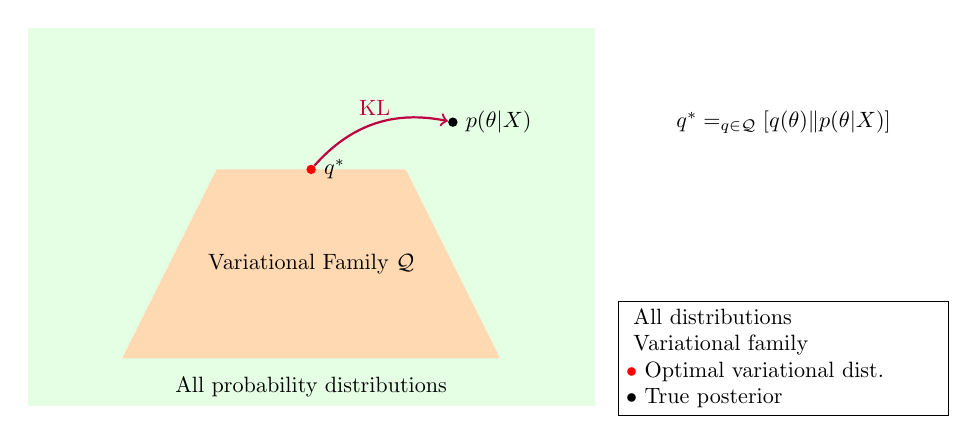
\begin{tikzpicture}[
			scale=1.2,
			every node/.style={scale=0.8}
		]
		% Draw the background rectangle
		\fill[green!10] (-3, -2) rectangle (3, 2);

		% Draw the variational family polygon (symmetric)
		\fill[orange!30] (-2, -1.5) -- (-1, 0.5) -- (1, 0.5) -- (2, -1.5) -- cycle;

		% Add labels
		\node at (5, 1) {$q^* = \argmin_{q \in \mathcal{Q}} \KL[q(\theta) \| p(\theta|X)]$};
		\node at (0, -0.5) {Variational Family $\mathcal{Q}$};
		\node at (0, -1.8) {All probability distributions};

		% Place q* and p(theta|X) points
		\node[fill=red, circle, inner sep=1.5pt, label=right:{$q^*$}] (q_star) at (0, 0.5) {};
		\node[fill=black, circle, inner sep=1.5pt, label=right:{$p(\theta|X)$}] (p_theta) at (1.5, 1) {};

		% Add KL divergence arrow
		\draw[->, thick, purple] (q_star) to[bend left] node[midway, above] {KL} (p_theta);

		% Add legend
		\node[draw, rectangle, text width=5cm, align=left] at (5, -1.5) {
			\textcolor{green!50!black}{$\square$} All distributions \\
			\textcolor{orange}{$\square$} Variational family \\
			\textcolor{red}{$\bullet$} Optimal variational dist. \\
			\textcolor{black}{$\bullet$} True posterior
		};
	\end{tikzpicture}
	\caption{Illustration of Bayesian posterior inference. The green background represents the space of all probability distributions, while the orange polygon represents the variational family $\mathcal{Q}$. The red point $q^*$ is the optimal variational distribution that minimizes the KL divergence to the true posterior $p(\theta|X)$, represented by the black point. The purple arrow indicates the KL divergence being minimized. This figure demonstrates the core concept of variational inference, where we approximate the true posterior with a simpler distribution from a restricted family, balancing computational tractability with inference accuracy.}
	\label{fig:bayesian_inference}
\end{figure}

\subbibliography{library.bib}
\end{document}